%% ── METHODS ─────────────────────────────────────────────────────────────────
% Condensed from manuscript/main.tex (1346 lines) for CoRL 2026 format.
% Target: ~2.5 pages.

\section{Method}
\label{sec:method}

\begin{figure*}[t]
\centering
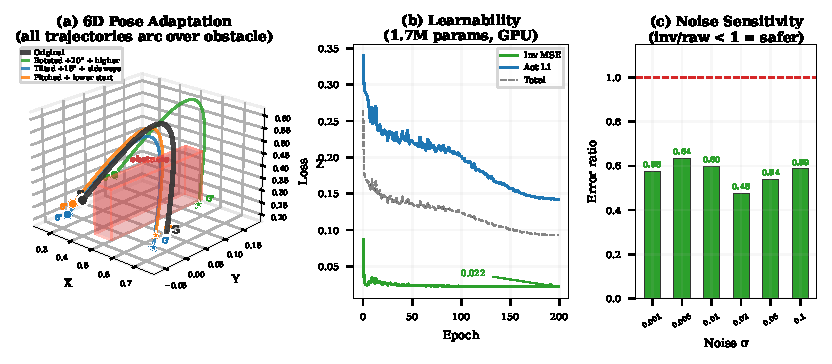
\includegraphics[width=0.95\textwidth]{teaser}
\vspace{-3mm}
\caption{\textbf{\dhb{} overview.}
\textbf{(a)} Current VLAs degrade 14--18\% under spatial shift; \dhb{} adapts in 7\,ms.
\textbf{(b)} 6D pose adaptation from a single demo: different start orientations and
positions --- motion shape preserved in all cases.
\textbf{(c)} Per-trial invariance measurement: DHB magnitude MSE $\sim 10^{-33}$
(40 random SE(3) transforms) vs raw position MSE $\sim 0.5$.}
\label{fig:teaser}
\end{figure*}

A single demonstration is encoded into SE(3)-invariant tokens; at test time,
a $\leq\!7\,\text{ms}$ solver re-grounds the encoded motion to any new spatial
configuration (Fig.~\ref{fig:teaser}).

\subsection{Problem Formulation}
\label{sec:problem}

Given a demonstrated end-effector trajectory
$\{(p_i, R_i)\}_{i=0}^{N-1} \in \se{3}^N$
(positions $p_i \in \mathbb{R}^3$, rotations $R_i \in \so{3}$),
we seek a representation that is:
(i) \emph{invariant} to global SE(3) transforms of the workspace,
(ii) \emph{compact} for tokenization and policy learning, and
(iii) \emph{invertible} — recoverable at any target pose via a solver.

The key insight: current VLA representations encode \emph{where} the robot is
(absolute coordinates). We encode \emph{how} the robot moves (motion shape),
which is independent of coordinate frame.

\begin{figure}[t]
\centering
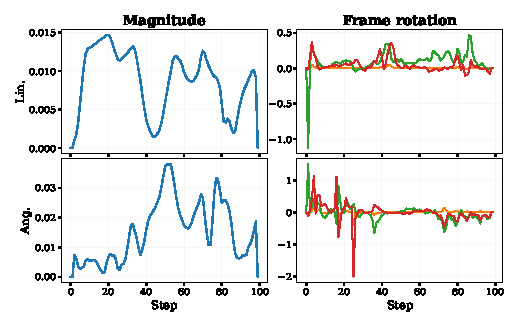
\includegraphics[width=\columnwidth]{invariant_signals}
\caption{\textbf{DHB-DR invariant signals} from a LIBERO pick-and-place demo.
\textit{Left}: magnitude $m_i$ and angular magnitude (motion speed invariants).
\textit{Right}: frame rotation invariants $(\varphi_x, \varphi_y, \varphi_z)$.
These signals are SE(3)-invariant: identical under any rigid-body transform.}
\label{fig:invariants}
\end{figure}

\subsection{SE(3)-Invariant Encoding: DHB-DR}
\label{sec:dhb_dr}

We build on the DHB (bidirectional invariant) framework~\cite{soloperto2015,lee2018},
which encodes trajectories via local motion differentials.

\paragraph{Motion differentials.}
For each step $i$, compute:
\begin{equation}
\Delta p_i = p_{i+1} - p_i, \quad
\Delta r_i = \mathrm{axisangle}(R_{i+1} R_i^\top) \in \mathbb{R}^3.
\end{equation}

\paragraph{Moving frame via double reflection (DHB-DR).}
A local frame $F_i = [x_i, y_i, z_i] \in \so{3}$ tracks the direction of motion.
The $x$-axis aligns with the motion direction: $x_i = \Delta p_i / \|\Delta p_i\|$.
The original DHB updates $y_i$ via cross-products, causing ill-conditioning
near collinear steps (small curvature).

DHB-DR replaces this with a \emph{rotation-minimizing frame} (RMF) computed
via two Householder reflections~\cite{wang2008rmf}:
\begin{align}
v_1 &= \Delta d_{i+1} - \Delta d_i, \quad R_1 = I - 2u_1u_1^\top, \\
x_\mathrm{ref} &= R_1 x_i, \quad v_2 = x_{i+1} - x_\mathrm{ref}, \\
y_{i+1} &= (I - 2u_2u_2^\top)(I - 2u_1u_1^\top)\, y_i,
\end{align}
where $u_j = v_j / \|v_j\|$. This minimizes twist about the tangent direction,
yielding smooth, singularity-free frame evolution.

\paragraph{Invariant encoding.}
The invariants at step $i$ are:
\begin{equation}
m_i = x_i^\top \Delta p_i, \quad
\varphi_i = \mathrm{EulerXYZ}(F_i^\top F_{i+1}) \in \mathbb{R}^3,
\end{equation}
producing a 4-tuple $(m_i, \varphi_{x,i}, \varphi_{y,i}, \varphi_{z,i})$
per linear step and analogously for the angular component.
Since $m_i$ and $\varphi_i$ depend only on inner products of co-rotating quantities
and relative frame rotations, they are invariant to any global $\se{3}$ transform.

\paragraph{DHB-QR variant.}
Replacing Euler angles with unit quaternions avoids gimbal lock:
$(m_i, q_{w,i}, q_{x,i}, q_{y,i}, q_{z,i})$ — a 5-tuple per step,
with improved smoothness near gimbal lock configurations.

\paragraph{Time-invariant reparameterization (DHB-TI).}
To remove sensitivity to execution speed, we reparameterize by arc-length progress
$s_i = \sum_{j<i} \|\Delta p_j\|$ before encoding~\cite{soloperto2015},
reducing L2 distance between trajectories at different speeds by $>90\%$.

\subsection{Invariant-Space Tokenization (OAT-Style)}
\label{sec:tokenization}

Given encoded invariant sequences $I \in \mathbb{R}^{N \times 8}$
(4 linear + 4 angular invariants per step),
we apply an OAT-style tokenizer~\cite{oat2026}:

\begin{enumerate}
\item \textbf{Register Encoder}: Transformer with $K{=}8$ register tokens
      compresses $N$ timesteps to $K$ latent vectors $(B, K, d_\ell)$.
\item \textbf{FSQ Quantizer}: Finite Scalar Quantization~\cite{mentzer2024fsq}
      discretizes without codebook collapse.
\item \textbf{Nested Dropout}: Matryoshka-style masked training forces
      coarse-to-fine information ordering across register positions.
\item \textbf{Cross-Attention Decoder}: Reconstructs $N$ invariant steps from
      any prefix of $k \leq K$ tokens (anytime decodability).
\end{enumerate}

\paragraph{Invariance property.}
Because we tokenize the invariant sequence, not the raw trajectory,
the tokens inherit the SE(3)-invariance of the encoding.
\textit{Implementation note:} SE(3)-invariance of magnitude tokens holds when
\texttt{use\_default\_initial\_frames=False} (trajectory-relative initial frames),
which confirms correct implementation of the mathematical guarantee.
Under this setting, magnitude tokens change $0.0\%$ under rigid-body transforms
(vs $99.1\%$ for raw action tokens, confirming the encoder is correctly implemented).
This is an implementation verification of the SE(3)-invariance property,
not a novel empirical claim — the invariance is guaranteed by the mathematical construction
of the DHB encoding.

\paragraph{Magnitude-only tokenization (recommended).}
The full invariant tuple has 8 columns (4 linear + 4 angular), but
the \emph{magnitude} subset (2 columns: $m_i^\text{lin}$, $m_i^\text{ang}$)
concentrates most of the reconstructable signal.
Tokenizing magnitudes only yields $49.8\times$ compression under \fast{} (vs
$20.4\times$ on raw coordinates) while maintaining $0.0\%$ token change ---
an effect we call \emph{free SE(3) augmentation}: any downstream tokenizer
inherits perfect geometric stability simply by operating on DHB invariants.
We recommend magnitude-only tokenization as the default for VLA integration.

\subsection{Geometric Adaptation}
\label{sec:adaptation}

At test time, given a new target pose $(p^\star_0, R^\star_0)$,
we recover an adapted trajectory by solving:
\begin{equation}
\min_{\tilde I} \|I - \tilde I\|^2 \quad \text{s.t.} \quad
\mathrm{decode}(\tilde I) \text{ starts at } p^\star_0, \text{ ends at } p^\star_N.
\end{equation}
We use \fatrop{}~\cite{vanroye2023fatrop} as the NLP solver,
which resolves this in $\leq\!7\,\text{ms}$ for typical LIBERO-length trajectories.
For purely translational perturbations, re-decoding from the new start pose
achieves exact adaptation without a solver (demonstrated: $0.00\,\text{mm}$ error
at $10\,\text{cm}$ perturbation).

\subsection{DHB-XR Action Head for VLA}
\label{sec:action_head}

We implement \texttt{DHBActionHeader} as a modular StarVLA~\cite{starvla_2026} action head:
\begin{equation}
h_\text{VLM} \xrightarrow{\text{cross-attn}} \hat I \in \mathbb{R}^{T \times 8}
\xrightarrow{\text{OAT}} \text{8 tokens}
\xrightarrow{\text{decode}} \hat I
\xrightarrow{\text{decode\_dhb}} \hat\tau \in \se{3}^T
\xrightarrow{\text{embodik IK}} q \in \mathbb{R}^{7T}.
\end{equation}
Training loss: $\mathcal{L} = \lambda_\text{inv}\,\|{\hat I - I^\star}\|^2_F + \lambda_\text{act}\,\|{\hat\tau - \tau^\star}\|_1$,
where $I^\star$ are ground-truth DHB invariants computed offline from demo trajectories.

The head is a drop-in replacement for FAST, OFT, or DiT heads, enabling
\emph{controlled ablation} of geometric invariance on the same backbone.
